\chapter{Evaluation}
\label{ch:evaluation}

This chapter evaluates whether the chunks produced by the library of
\cref{ch:implementation} are retrieved more accurately than those of the baseline
strategies. After the datasets (\cref{sec:datasets}) and the design (\cref{sec:design}),
\cref{sec:results} reports the main comparison;
\cref{sec:further} examines the source of the
differences, the low-information filter and the other configuration options and
parent-child retrieval, and \cref{sec:threats} discusses robustness and validity. \Cref{ch:lessons} interprets the results.

\section{Datasets and question sets}
\label{sec:datasets}

The evaluation uses three documents, one for each structure class of
\cref{sec:commitments} (\cref{tab:datasets}).

\begin{table}[htbp]
  \centering
  \caption{Evaluation documents. Characters after text extraction, sentences as counted by
  the library's sentence splitter, and questions that passed the verification
  (\cref{sec:questions}).}
  \label{tab:datasets}
  \small
  \begin{tabular}{@{}lL{5.4cm}lrrr@{}}
    \toprule
    Document & Source and format & Structure class & Characters & Sentences & Questions \\
    \midrule
    \code{rfc9110} & RFC 9110, HTTP Semantics~\cite{rfc9110}; plain text & explicit & \num{502906} & \num{3882} & 549 \\
    \code{nasa}    & NASA Systems Engineering Handbook~\cite{nasa2016handbook}; PDF, 297 pages & implicit & \num{813744} & \num{6071} & 534 \\
    \code{wells}   & H.\,G.~Wells, \emph{A Short History of the World}~\cite{wells1922history}; plain text & unstructured & \num{616390} & \num{4754} & 400 \\
    \bottomrule
  \end{tabular}
\end{table}

\code{rfc9110} is an explicit text: a technical standard with numbered sections
throughout. \code{wells} is continuous narrative prose about different historical periods,
in which the topic shifts are fluid throughout the document. \code{nasa} (NASA
SP-2016-6105 Rev2) changes topic from paragraph to paragraph, but loses its layout during
text extraction. The project's PDF reader joins the lines of a page into one paragraph
(310 paragraphs, median \num{2830} characters), and the running header appears inside the
text on almost every page.

\paragraph{Question sets.}
\label{sec:questions}
The questions were generated by an external language model (Claude Sonnet 5), never by the
local model under test. The prompt requires every question to come with an anchor: a
passage of 60 to 300 characters, copied verbatim from the document, that contains the
answer. Furthermore, the prompt requires a question to be answerable from one section
alone and its anchor to appear only once in the text. An automatic check
(\cref{sec:verify-questions}) then tests every candidate against the extracted text: the
anchor must be verbatim after normalisation, at least 40 characters long, not duplicated
and unique in the document. Candidates that fail are discarded (16 of 550 on \code{nasa},
4 of 553 on \code{rfc9110}). No questions were removed or added by hand afterwards.

\section{Experimental design}
\label{sec:design}

\subsection{Compared strategies}

The LLM chunker is evaluated in two arms that share one configuration: two sentences per
decision (\code{step\_sentences=2}), a size cap of \num{1200} characters, at most 100
sentences per chunk and no heading detection. The \emph{tested arm} also switches off the
low-information filter, which the library enables by default, so that it evaluates the
chunking alone, without any post-processing. The \emph{filter arm} is the same
configuration with the filter; it shows the effect of the filter as an optional add-on
(\cref{sec:filter}) and is the reference for the ablations (\cref{sec:ablations}).
\Cref{tab:strategies} lists the five baselines.

\begin{table}[htbp]
  \centering
  \caption{Baselines. All are length-matched to the LLM chunker (see text).}
  \label{tab:strategies}
  \small
  \begin{tabular}{@{}L{3.2cm}L{11.3cm}@{}}
    \toprule
    Strategy & Implementation \\
    \midrule
    Fixed-size & LangChain \code{CharacterTextSplitter}, space as separator, overlap of 50 characters. \\
    Recursive (default) & LangChain \code{RecursiveCharacterTextSplitter} with its default separator order: paragraph, line break, space. A paragraph longer than the target is cut at the last space that fits, usually inside a sentence. Overlap of 50 characters. \\
    Recursive (sentence ends) & The same class with a sentence end (whitespace after \code{.}, \code{!} or \code{?}) as second separator, before line break and space, so that an over-long paragraph is cut after the last complete sentence that fits. Overlap of 50 characters. \\
    Semantic (tuned) & LangChain \code{SemanticChunker} with the same bge-m3 embeddings. The percentile threshold is set by bisection to reach the target length, and chunks above \num{1200} characters are divided at sentence boundaries. \\
    Packing (no model) & The library's own \code{LLMChunker} with a stand-in client that always answers \enquote{same topic}, so that every boundary comes from the size cap, which cuts between sentences (at the middle sentence). \\
    \bottomrule
  \end{tabular}
\end{table}

\paragraph{Length matching.} Because chunk length can influence the hit rates, every
baseline is tuned to the mean length of the LLM chunks that the filter keeps (714
characters on \code{nasa}, 720 on \code{rfc9110}, 725 on \code{wells}). The tested arm's
own mean is lower (454, 621 and 711 characters), because it also contains the chunks that
the filter removes, mostly short fragments such as 464 chunks of the \code{nasa} table of
contents that consist of nothing but dot leaders. A splitter's mean length cannot be set
directly, so its parameters (chunk size, percentile threshold etc.) are adjusted until the
mean lies within \SI{4}{\percent} of the target.

\subsection{Retrieval, hit criterion and statistical analysis}
\label{sec:stats}

Chunks and questions are embedded with bge-m3~\cite{chen2024bgem3}, served by a local
Ollama instance. Retrieval uses exact search: each question is compared with every chunk
by cosine similarity, and the chunks are ranked by this score. The approximate HNSW
index~\cite{malkov2020hnsw} that the project's vector store uses by default does not
guarantee the true nearest neighbours; in this project, its ranking changed each time the
same data was indexed again, so it was not used for the final results.

Each question is judged by how much of its anchor is present in a chunk. A question counts
as a hit at rank $k$ (\hitk{k}) if one of the $k$ highest-ranked chunks contains at least
\SI{80}{\percent} of the anchor as one continuous passage. The threshold accepts an anchor
whose last words fall into the next chunk, but not one that a chunk boundary splits in
half. Line breaks and repeated spaces are ignored, so that formatting differences between
document and chunks do not matter, and the passage must be continuous, so that a chunk
does not count merely because it shares words with the anchor. Applied to all chunks of a
strategy instead of only the top $k$, the same test gives the share of \emph{anchors
intact}: if no chunk contains at least \SI{80}{\percent} of the anchor, the chunking has
cut the answer apart and no retriever can find it. This share is therefore an upper bound
for \hitk{k} at every $k$. \hitk{1} and \hitk{3} are the reported metrics.

A potential downside of this approach is that the hit criterion favours large chunks: the larger a chunk, the more likely it is to
contain a given anchor, and with one chunk per document every question would be a hit at
$k=1$. However, two measures prevent this effect from deciding the comparison. First, all
baselines are length-matched to the LLM chunker (\cref{sec:design}), so that no strategy
has larger chunks on average and the remaining differences stem from where the boundaries
are placed, not from how large the chunks are. Second, the LLM chunker and the tuned
semantic chunker are limited by a size cap of \num{1200} characters, so that no chunk can
span large parts of a document. In practice, such chunks would also be of little use,
since they dilute the embedding and fill the context of the generating model with
irrelevant text (\cref{sec:rag_chunking}), which would lead to worse answer generation.

\paragraph{Statistical analysis.} All strategies are evaluated on the same questions, so they
can be compared question by question. When the tested arm is compared with one baseline, only the questions on which
the two disagree are informative: $b$ is the number of questions that only the LLM arm
answers, and $c$ the number that only the baseline answers. Questions that both or neither
answer are ignored. If both strategies were equally good, each of these disagreements
would go to the LLM arm or to the baseline with a probability of $1/2$. The exact McNemar
test~\cite{mcnemar1947} computes the two-sided probability $p$ of a split at least as
uneven as the observed one under this assumption. The size of the effect is the
difference in hit rate, $d = (b-c)/n$ with $n$ questions, in percentage points (pp), with a
\SI{95}{\percent} Wald interval for paired proportions,
$d \pm 1.96\sqrt{\bigl((b+c)/n - d^2\bigr)/n}$, which gives the range of differences
compatible with the data; an interval that contains zero means that no difference can be
established. The intervals are not adjusted for multiple testing.

The tested arm is compared with five baselines on three documents at two values of $k$,
which gives a total of 30 tests. Holm's procedure~\cite{holm1979} controls the family-wise
error rate, the probability of at least one false positive among the 30 tests, at
$\alpha = 0.05$: the $p$-values are sorted in ascending order, the $i$-th smallest is
compared with $\alpha/(30-i+1)$, and the procedure stops at the first comparison that
fails. Equivalently, the $i$-th smallest $p$-value is multiplied by $30-i+1$, capped at 1
and never allowed to fall below the adjusted value before it; these \emph{adjusted}
$p$-values are reported and can be compared with $\alpha$ directly, whereas
\emph{unadjusted} values refer to a single test.

\section{Results}
\label{sec:results}

\begin{table}[htbp]
  \centering
  \caption{Hit rates in percent. The tested arm is compared with the five baselines;
  the filter arm with the low-information filter as an add-on is shown for reference
  (\cref{sec:filter}).}
  \label{tab:results}
  \small
  \begin{tabular}{@{}lrrrrrr@{}}
    \toprule
    & \multicolumn{2}{c}{\code{nasa} ($n=534$)} & \multicolumn{2}{c}{\code{rfc9110} ($n=549$)} & \multicolumn{2}{c}{\code{wells} ($n=400$)} \\
    \cmidrule(lr){2-3}\cmidrule(lr){4-5}\cmidrule(l){6-7}
    Strategy & \hitk{1} & \hitk{3} & \hitk{1} & \hitk{3} & \hitk{1} & \hitk{3} \\
    \midrule
    LLM (tested arm) & 69.5 & 87.1 & 74.9 & 90.2 & 84.0 & 92.8 \\
    Recursive (sentence ends) & 66.9 & 84.3 & 71.6 & 88.0 & 89.8 & 96.2 \\
    Packing (no model) & 64.8 & 82.6 & 71.6 & 87.4 & 86.5 & 94.8 \\
    Semantic (tuned) & 66.5 & 83.3 & 73.6 & 89.8 & 83.2 & 93.8 \\
    Recursive (default) & 61.6 & 80.3 & 71.8 & 88.0 & 87.2 & 95.0 \\
    Fixed-size & 61.2 & 76.8 & 58.5 & 80.5 & 77.8 & 89.8 \\
    \addlinespace
    LLM with filter (add-on) & 68.0 & 83.5 & 73.6 & 88.3 & 84.0 & 92.8 \\
    \bottomrule
  \end{tabular}
\end{table}

\Cref{tab:results} shows a pattern that the individual tests confirm. On \code{nasa} and
\code{rfc9110}, the tested arm reaches the highest hit rates of the six compared
strategies at both $k$ (\hitk{1} \SI{69.5}{\percent} and \SI{74.9}{\percent}), but it
leads the sentence-aware baselines by only 0.4 to 4.7~pp. On \code{wells}, three baselines
are ahead of it; the clear winner, the recursive splitter with sentence ends, reaches
\SI{89.8}{\percent} against \SI{84.0}{\percent}. Fixed-size splitting is the weakest
strategy on every document. At $k=3$, most differences on \code{rfc9110} and \code{wells}
shrink, because a passage missed at rank~1 is often found at rank~2 or~3.

\begin{figure}[htbp]
  \centering
  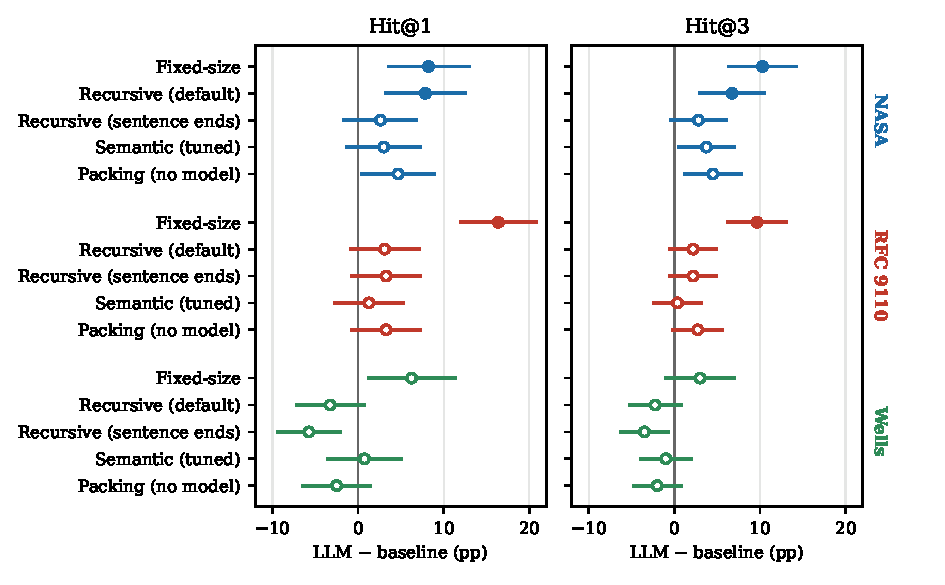
\includegraphics[width=\textwidth]{figures/forest_v4.pdf}
  \caption{Difference in hit rate between the tested LLM arm and each baseline, with
  \SI{95}{\percent} intervals. Filled markers are significant after the Holm correction
  over all 30 tests. Values right of zero favour the LLM chunker.}
  \label{fig:forest}
\end{figure}

Six of the 30 comparisons remain significant after the Holm correction, all against the
two naive splitters. Against fixed-size splitting, the tested arm leads on \code{rfc9110}
by $+16.4$~pp at \hitk{1} [$+12.0$, $+20.8$] and $+9.7$~pp at \hitk{3} [$+6.2$, $+13.1$],
and on \code{nasa} by $+8.2$ and $+10.3$~pp (adjusted $p \le 0.021$). Against LangChain's
default recursive splitter, it leads on \code{nasa} by $+7.9$~pp at \hitk{1} [$+3.2$,
$+12.5$] and $+6.7$~pp at \hitk{3} (adjusted $p = 0.030$ and $0.014$). The nearest miss is
in the opposite direction: the lead of the recursive splitter with sentence ends on
\code{wells} ($-5.8$~pp at \hitk{1}), which is not significant after the Holm correction
(adjusted $p = 0.064$).

\Cref{fig:forest} makes the structure of the result visible. Against fixed-size splitting,
all four intervals on \code{nasa} and \code{rfc9110} lie above zero; against the default
recursive splitter, the two on \code{nasa} do. Against the three baselines that keep
sentences intact (recursive with sentence ends, the tuned semantic chunker and packing
without the model), the point estimates on \code{nasa} and \code{rfc9110} lie between
$+0.4$ and $+4.7$~pp, and nine of the twelve intervals contain zero. On \code{wells}, the
LLM arm is behind three of the five baselines at \hitk{1} and four at \hitk{3}.

\section{Further analyses}
\label{sec:further}

\subsection*{Where the differences come from}
\label{sec:mechanism}

\begin{table}[htbp]
  \centering
  \caption{Chunks ending inside a sentence (mid-sent.) and anchors contained to at least
  \SI{80}{\percent} in some chunk (intact), in percent.}
  \label{tab:mechanism}
  \small
  \begin{tabular}{@{}lrrrrrr@{}}
    \toprule
    & \multicolumn{2}{c}{\code{nasa}} & \multicolumn{2}{c}{\code{rfc9110}} & \multicolumn{2}{c}{\code{wells}} \\
    \cmidrule(lr){2-3}\cmidrule(lr){4-5}\cmidrule(l){6-7}
    Strategy & mid-sent. & intact & mid-sent. & intact & mid-sent. & intact \\
    \midrule
    LLM (tested arm) & 3.1 & 98.7 & 11.9 & 99.3 & 7.1 & 95.0 \\
    Recursive (sentence ends) & 19.3 & 98.9 & 35.2 & 99.6 & 16.0 & 99.5 \\
    Packing (no model) & 3.8 & 98.1 & 18.3 & 98.9 & 3.4 & 96.2 \\
    Semantic (tuned) & 3.4 & 97.9 & 6.5 & 98.9 & 1.2 & 95.8 \\
    Recursive (default) & 83.7 & 94.6 & 37.6 & 99.5 & 34.6 & 98.0 \\
    Fixed-size & 94.8 & 92.1 & 93.0 & 93.1 & 96.7 & 93.8 \\
    \addlinespace
    LLM with filter (add-on) & 4.0 & 93.6 & 9.2 & 97.3 & 6.0 & 95.0 \\
    \bottomrule
  \end{tabular}
\end{table}

The anchors are one or two sentences long, so a chunking that never cuts inside a sentence
keeps almost every anchor intact, whatever it does between sentences. \Cref{tab:mechanism}
shows the proportion of chunks that end without sentence-final punctuation, a proxy for a
cut inside a sentence. Fixed-size splitting ends 93 to \SI{97}{\percent} of its chunks
inside a sentence and leaves only 92 to \SI{94}{\percent} of the anchors intact.
LangChain's default recursive splitter performs better on \code{rfc9110} and \code{wells},
whose paragraphs are short, but on \code{nasa} it finds no paragraph break within the
target length and falls back to the space character, so that \SI{83.7}{\percent} of its
chunks end inside a sentence. This is where the LLM arm is furthest ahead, although the
situation is created primarily by the text extraction rather than by the document.

The strongest evidence on the contribution of the model comes from packing, which uses the
same sentence splitter and assembly loop without asking the model anything. It trails the
tested arm by 4.7~pp on \code{nasa} and 3.3~pp on \code{rfc9110} at \hitk{1}, neither
difference significant after the correction, and leads it by 2.5~pp on \code{wells}. On
\code{wells}, \SI{77}{\percent} of the LLM arm's boundaries are forced by the size cap
rather than set by a topic decision (on \code{nasa} \SI{46}{\percent}, on \code{rfc9110}
\SI{53}{\percent}), so there the chunker behaves largely like packing with a different
split point. The model's topic decisions produce boundaries that differ from packing, but
no retrieval benefit that remains significant after the correction.

\subsection*{The low-information filter and other options}
\label{sec:filter}

This section evaluates the optional features of the library: the low-information filter
as an add-on to the tested arm, and three further options as single-setting ablations.

\paragraph{Low-information filter.} The filter is an optional post-processing step: after
chunking, the model judges every chunk, and the ones without substantive information are removed. Added to the tested
configuration, it drops 761 of \num{1786} chunks on \code{nasa} but only
\SI{9.8}{\percent} of the text, mostly fragments such as the dot leaders of the table of
contents. It also deletes answers: 27 anchors of \code{nasa} and 11 of \code{rfc9110} are
no longer contained in any chunk. On \code{nasa}, 18 of these 27 lie in the reference
lists, from which the generating model produced 35 questions although the prompt excluded
them. As a result, the filter lowers \hitk{3} by 3.6~pp on \code{nasa} and by 1.8~pp on
\code{rfc9110} (Holm-adjusted $p = 0.002$ and $0.032$ over the six tests of this
comparison) and leaves \code{wells} unchanged.

The filter arm, tested against the five baselines with its own Holm family of 30 tests,
keeps only two significant results, both against fixed-size splitting on \code{rfc9110}
($+15.1$ and $+7.8$~pp). Its leads over the naive splitters on \code{nasa} at \hitk{1}
($+6.4$~pp against the default recursive splitter, $+6.7$~pp against fixed-size splitting)
are no longer significant (adjusted $p = 0.28$ and $0.18$), mainly because the filter
deletes passages that some questions ask about.

\label{sec:ablations}
Three further options of \cref{ch:implementation} were evaluated as single-setting changes
of the filter arm, the tested arm of the original design, produced in the same chunking run and
scored on the same questions. These comparisons are exploratory only; none of the
differences would survive a correction for multiple testing (the smallest unadjusted $p$
is 0.029).

\paragraph{Split point at the size cap.} Splitting an over-long chunk at its middle
sentence instead of at the point chosen by the model (\code{nasa} only) changes \hitk{1}
by $-0.2$~pp and \hitk{3} by $-2.2$~pp ($p = 0.13$).

\paragraph{Heading detection.} Neither heading mode (line pattern or hybrid with the
model) changes a hit rate by more than 0.7~pp on any document. On \code{wells}, the
line-pattern arm is identical to the reference, and on \code{nasa}, whose line structure
is lost in extraction, the chunk lists differ from the reference by only 7 (line pattern)
and 52 (with the model) chunks, so that heading detection has little to change on these
two documents.

\paragraph{Topic enrichment.} A model-generated topic line in front of each chunk lowers
\hitk{1} on all three documents ($-0.9$, $-2.2$ and $-1.8$~pp) and \hitk{3} as well. The
label therefore does not help the retriever find the passage.

\subsection*{Parent-child retrieval}
\label{sec:parentchild}

The evaluation harness also implements parent-child retrieval, a retrieval technique that
is independent of the chunking and is used here as an additional condition under which the
strategies are compared. Every chunk (the parent) is divided into children of 250
characters (with LangChain's recursive splitter and an overlap of 30 characters), the
children are embedded and searched, and the parents of the best children are returned,
each parent at most once. It was applied to the tested arm and to all five baselines, with
the same questions, search and hit criterion as in \cref{sec:results}.

\begin{table}[htbp]
  \centering
  \caption{Hit rates in percent with parent-child retrieval, applied to every strategy.
  In parentheses: change of \hitk{1} against the same strategy without parent-child
  (\cref{tab:results}), in pp.}
  \label{tab:parentchild}
  \small
  \begin{tabular}{@{}lrrrrrr@{}}
    \toprule
    & \multicolumn{2}{c}{\code{nasa}} & \multicolumn{2}{c}{\code{rfc9110}} & \multicolumn{2}{c}{\code{wells}} \\
    \cmidrule(lr){2-3}\cmidrule(lr){4-5}\cmidrule(l){6-7}
    Strategy & \hitk{1} & \hitk{3} & \hitk{1} & \hitk{3} & \hitk{1} & \hitk{3} \\
    \midrule
    LLM (tested arm) & 72.5 ($+3.0$) & 88.4 & 80.0 ($+5.1$) & 91.1 & 86.2 ($+2.2$) & 92.5 \\
    Recursive (sentence ends) & 73.0 ($+6.2$) & 87.6 & 82.9 ($+11.3$) & 92.7 & 90.0 ($+0.2$) & 97.5 \\
    Packing (no model) & 73.0 ($+8.2$) & 86.0 & 76.3 ($+4.7$) & 91.6 & 85.5 ($-1.0$) & 93.2 \\
    Semantic (tuned) & 71.2 ($+4.7$) & 88.2 & 77.6 ($+4.0$) & 90.5 & 89.0 ($+5.8$) & 94.5 \\
    Recursive (default) & 64.2 ($+2.6$) & 81.1 & 82.7 ($+10.9$) & 92.5 & 89.2 ($+2.0$) & 96.2 \\
    Fixed-size & 57.9 ($-3.4$) & 73.6 & 71.8 ($+13.3$) & 83.6 & 78.8 ($+1.0$) & 89.8 \\
    \bottomrule
  \end{tabular}
\end{table}

Parent-child raises most hit rates, but not evenly (\cref{tab:parentchild}), and the
baseline splitters gain the most on average. On \code{rfc9110}, the rule-based splitters
gain the most at \hitk{1} (fixed-size $+13.3$~pp, the two recursive splitters $+10.9$ and
$+11.3$~pp, against $+5.1$~pp for the LLM arm). On \code{nasa}, packing and the splitter
with sentence ends gain $+8.2$ and $+6.2$~pp against $+3.0$~pp for the LLM arm. On
\code{wells}, the changes are small except for the semantic chunker ($+5.8$~pp).

With parent-child applied to every strategy, the balance against the sentence-aware
baselines shifts towards the baselines. The recursive splitter with sentence ends combined
with parent-child retrieval reaches a higher \hitk{1} than the LLM chunker with or without
it on all three documents (\SI{73.0}{\percent}, \SI{82.9}{\percent} and
\SI{90.0}{\percent}), at no cost in model calls. Tested in the same way as in
\cref{sec:results}, with parent-child on both sides, the LLM arm remains significantly
ahead only of the two naive splitters (four tests on \code{nasa}, two on \code{rfc9110})
and is significantly behind the recursive splitter with sentence ends on \code{wells} at
\hitk{3} ($-5.0$~pp, adjusted $p = 0.040$).

\section{Robustness and threats to validity}
\label{sec:threats}

\label{sec:robustness}
The hit rates of all arms in \cref{tab:results} and the 30 tests of the filter arm were
recomputed by a second, independent implementation of the search, the hit criterion and
the tests, with identical results. \Cref{tab:sensitivity} shows how the result depends on
analysis decisions. The absence of a significant lead over the sentence-aware baselines
holds in every variant, and so does the lead over fixed-size splitting on \code{rfc9110}.
The lead over the naive splitters on \code{nasa} is less stable: it disappears when the
filter is added, and without the 35 questions from the reference lists, an exclusion
decided after seeing the results and therefore reported only as a sensitivity analysis,
the lead over the default recursive splitter at \hitk{1} is no longer significant,
although the one at \hitk{3} is.

\begin{table}[htbp]
  \centering
  \caption{Dependence of the result on analysis decisions. The \code{nasa} columns give
  the difference at \hitk{1} in pp with the Holm-adjusted $p$ in parentheses; the last
  column counts significant leads of the LLM arm over a sentence-aware baseline.}
  \label{tab:sensitivity}
  \small
  \begin{tabular}{@{}L{5.0cm}crrc@{}}
    \toprule
    & & \multicolumn{2}{c}{\code{nasa}, \hitk{1}} & \\
    \cmidrule(lr){3-4}
    Variant & Significant & vs.\ recursive & vs.\ fixed-size & Sentence-aware \\
    \midrule
    Main analysis (tested arm) & 6 of 30 & $+7.9$ (\textbf{0.030}) & $+8.2$ (\textbf{0.021}) & none \\
    Tested arm without the 35 reference-list questions (post hoc) & 5 of 30 & $+7.4$ (0.067) & $+8.0$ (\textbf{0.038}) & none \\
    Filter arm (original design) & 2 of 30 & $+6.4$ (0.279) & $+6.7$ (0.176) & none \\
    Filter arm without the 35 reference-list questions (post hoc) & 6 of 30 & $+8.2$ (\textbf{0.024}) & $+8.8$ (\textbf{0.012}) & none \\
    \bottomrule
  \end{tabular}
\end{table}

\paragraph{Internal validity.} The questions were generated by a language model, and 35 of
the \code{nasa} questions violate the generation rules, but they were kept because the
procedure fixed in advance allowed no manual removal. Exact search, the length target, the
additional baselines and the size of the test family were decided after the first test
runs were known (\cref{sec:lessons}), with the intention of making the comparison fairer.
The choice of the filter-free configuration as tested arm was made after the final results
were known and raises the number of significant tests from two to six, but both results
(with and without the filter) are reported. In addition, the fixed-size and default
recursive splitters use an overlap of 50 characters, whereas the other strategies use
none. The tested and the filter arm were chunked in two separate runs.

\paragraph{External validity.} Each structure class is represented by one document, so
class and document cannot be separated. \code{nasa} is the only PDF, and its extraction
favours every sentence-aware strategy there. One chunking model, one embedding model and
one parameter setting were evaluated.

\paragraph{Evaluation validity.} \hitk{$k$} on verbatim anchors measures whether the
passage containing the answer is retrieved intact, not whether an LLM answers correctly
based on the retrieved chunk or whether a chunk reads coherently. A chunking strategy that
keeps topics together but splits an anchor passage can therefore be penalised.
